% !TeX program = xelatex
\documentclass[a4paper,12pt]{article}
% Личная преамбула и титульный лист; заполнить поля текущей работы.
\newcommand{\LabSubject}{Системы искусственного интеллекта}
\newcommand{\LabWorkType}{ЛАБОРАТОРНАЯ РАБОТА}
\newcommand{\LabNumber}{2}
\newcommand{\LabTopic}{Регуляризация и метод ближайших соседей}
\newcommand{\LabAuthor}{Михайлов Петр Сергеевич}
\newcommand{\LabGroup}{P3311}
\newcommand{\LabTeacher}{Королёва Юлия Александровна}
\newcommand{\LabYear}{2026}

\usepackage{iftex}
\ifPDFTeX
  \usepackage[T2A]{fontenc}
  \usepackage[utf8]{inputenc}
  \usepackage[russian]{babel}
\else
  \usepackage{fontspec}
  \usepackage{polyglossia}
  \setdefaultlanguage{russian}
  \setotherlanguage{english}
  \IfFontExistsTF{Times New Roman}{%
    \setmainfont{Times New Roman}\newfontfamily\cyrillicfont{Times New Roman}}{%
    \IfFontExistsTF{NimbusRoman-Regular.otf}{%
      \setmainfont{NimbusRoman}[Extension=.otf,UprightFont=*-Regular,BoldFont=*-Bold,ItalicFont=*-Italic,BoldItalicFont=*-BoldItalic]
      \newfontfamily\cyrillicfont{NimbusRoman}[Extension=.otf,UprightFont=*-Regular,BoldFont=*-Bold,ItalicFont=*-Italic,BoldItalicFont=*-BoldItalic]
    }{\setmainfont{DejaVu Serif}\newfontfamily\cyrillicfont{DejaVu Serif}}}
  \IfFontExistsTF{DejaVu Sans}{\setsansfont{DejaVu Sans}\newfontfamily\cyrillicfontsf{DejaVu Sans}}{\setsansfont{Arial}\newfontfamily\cyrillicfontsf{Arial}}
  \IfFontExistsTF{DejaVu Sans Mono}{\setmonofont{DejaVu Sans Mono}\newfontfamily\cyrillicfonttt{DejaVu Sans Mono}}{\setmonofont{Consolas}\newfontfamily\cyrillicfonttt{Consolas}}
\fi
\usepackage{amsmath,amssymb,amsfonts}
\usepackage{graphicx,geometry,listings,xcolor,hyperref,float,booktabs}
\usepackage{longtable,array,tabularx,caption}
\usepackage{tikz,pgfplots}
\usetikzlibrary{arrows.meta,fit,positioning}
\pgfplotsset{compat=1.18}
\geometry{left=2cm,right=1.5cm,top=2cm,bottom=2cm}
\hypersetup{unicode=true,colorlinks=true,linkcolor=black,citecolor=black,urlcolor=blue!60!black,
 pdftitle={\LabWorkType\space №\LabNumber. \LabTopic},pdfauthor={\LabAuthor}}
\captionsetup{font=small,labelsep=period}
\setlength{\parindent}{1.25cm}
\setlength{\parskip}{.2em}
\linespread{1.05}
\raggedbottom
\setcounter{tocdepth}{2}
\setlength{\emergencystretch}{2em}
\tolerance=3000
\lstdefinestyle{mypython}{language=Python,basicstyle=\ttfamily\scriptsize,
 keywordstyle=\color{blue!65!black}\bfseries,stringstyle=\color{red!65!black},
 commentstyle=\color{green!35!black},numbers=left,numberstyle=\tiny\color{gray},
 stepnumber=1,numbersep=7pt,showstringspaces=false,tabsize=4,frame=single,
 breaklines=true,breakatwhitespace=false,columns=fullflexible,keepspaces=true,
 xleftmargin=14pt,framexleftmargin=10pt,backgroundcolor=\color{gray!3}}
\lstset{style=mypython}

\graphicspath{{figures/}{docs/figures/}}
\begin{document}
\begin{titlepage}
\centering
{\fontsize{11}{13}\selectfont\textbf{Министерство науки и высшего образования Российской Федерации}}\\
{\fontsize{7}{10}\selectfont ФЕДЕРАЛЬНОЕ ГОСУДАРСТВЕННОЕ АВТОНОМНОЕ ОБРАЗОВАТЕЛЬНОЕ УЧРЕЖДЕНИЕ ВЫСШЕГО ОБРАЗОВАНИЯ}\\
\vspace{.2cm}
{\fontsize{14}{17}\selectfont\textbf{«НАЦИОНАЛЬНЫЙ ИССЛЕДОВАТЕЛЬСКИЙ УНИВЕРСИТЕТ ИТМО»}}
\vspace{1cm}

{\fontsize{12}{14}\selectfont\textbf{Факультет программной инженерии и компьютерной техники}}
\vspace{1cm}

{\fontsize{12}{14}\selectfont\textbf{Дисциплина: \LabSubject}}
\vspace*{\fill}

{\fontsize{18}{22}\selectfont\textbf{\LabWorkType\ №\,\LabNumber}}\\
\vspace{.5cm}
{\fontsize{14}{17}\selectfont\textbf{по теме: «\LabTopic»}}
\vspace{1.5cm}

\begin{flushright}
\fontsize{12}{14}\selectfont
Выполнил:\\
\LabAuthor\\
Группа: \LabGroup\\[1em]
Преподаватель:\\
\LabTeacher
\end{flushright}
\vfill
{\fontsize{12}{14}\selectfont Санкт-Петербург, \LabYear}
\end{titlepage}
\setcounter{page}{2}
{\small\setlength{\parskip}{0pt}\tableofcontents}
\newpage

\section{Цель и исходные данные}

Исследуем влияние штрафов L1, L2 и ElasticNet на линейную и логистическую регрессии. Для метода $k$ ближайших соседей (KNN) проверяем влияние расстояния, числа соседей и стандартизации на классификацию и регрессию.
Код и ноутбук размещаются в \href{https://github.com/Axe-On-You/Artificial-intelligence-systems/tree/main/\%D0\%9B\%D0\%B0\%D0\%B1\%D0\%BE\%D1\%80\%D0\%B0\%D1\%82\%D0\%BE\%D1\%80\%D0\%BD\%D0\%B0\%D1\%8F\%202}{папке лабораторной на GitHub}.

\begin{table}[H]
\centering
\caption{Цели и размеры выборок}
\label{tab:data}
\small
\begin{tabular}{llrrr}
\toprule
Набор & Целевая переменная & Train & Validation & Test \\
\midrule
Bike Sharing & \texttt{cnt} & 438 & 146 & 147 \\
Spaceship Titanic & \texttt{Transported} & 5\,215 & 1\,739 & 1\,739 \\
Dry Bean & \texttt{Class} & 8\,121 & 2\,710 & 2\,712 \\
Seoul Bike & \texttt{Rented Bike Count} & 5\,256 & 1\,752 & 1\,752 \\
\bottomrule
\end{tabular}
\end{table}

Для случайных разбиений из таблицы~\ref{tab:data} использован seed 5267. Spaceship Titanic и Dry Bean разделены стратифицированно по целевому классу. Seoul Bike разделён хронологически, все часы одного дня входят в одну выборку. Параметры преобразований определены по train, гиперпараметры выбраны по validation. Test используется для итоговой оценки.

\section{Регуляризация регрессий}

\subsection{Предобработка и функция потерь}

В Bike Sharing~\cite{bike} цель равна суточному числу аренд. Её слагаемые \texttt{casual} и \texttt{registered} исключены из признаков вместе с датой и номером строки. Погодные признаки стандартизированы, календарные и погодные категории кодируются one-hot. Для Spaceship Titanic~\cite{ship} цель бинарная. Из номера каюты выделены палуба, номер и сторона. Числовые пропуски заполнены медианами train, к расходам применён $\log(1+x)$, затем числовые признаки стандартизированы. Категориальные пропуски кодируются уровнем \texttt{Unknown}. Идентификатор пассажира и имя исключены. В каждой задаче после преобразований 33 признака.

Для матрицы признаков $X$, весов $w$ и свободного члена $b$ модель вычисляет $z=Xw+b$. Линейная регрессия минимизирует MSE для прогноза $z$, логистическая — BCE для вероятности $p=\sigma(z)$. Полная целевая функция
\begin{equation}
J(w,b)=L_{\text{data}}(w,b)+\lambda_1\sum_j |w_j|+\lambda_2\sum_j w_j^2 .
\label{eq:objective}
\end{equation}
Пары $(0,0)$, $(\lambda_1,0)$, $(0,\lambda_2)$ и $(\lambda_1,\lambda_2)$ при положительных $\lambda$ задают четыре режима сравнения. Градиенты $L_{\text{data}}$ по $w$ равны $2X^\top(z-y)/n$ для MSE и $X^\top(p-y)/n$ для BCE, где $n$ — размер train. Из~\eqref{eq:objective} получаем добавку
\begin{equation}
g_j=\lambda_1\operatorname{sign}(w_j)+2\lambda_2w_j.
\label{eq:gradient}
\end{equation}
При $w_j=0$ выбирается нулевой субградиент $|w_j|$. Свободный член обновляется по среднему $2(z-y)$ для MSE или $p-y$ для BCE. Тензорные вычисления и обновления выполняются в PyTorch. Качество на validation оценивается по RMSE и LogLoss соответственно.

\subsection{Выбор числа эпох и коэффициентов}

Пробные запуски без штрафа сравнивают шаги 0,01 и 0,03 для Bike Sharing, 0,05 и 0,1 для Spaceship Titanic. На рис.~\ref{fig:epochs} отмечены результаты на эпохах 100, 250, 500, 1000, 1500 и 2500. Общий бюджет для каждого набора определяется самой ранней эпохой с ошибкой в пределах 0,2\% от минимума по проверенным парам. При совпадении эпох выбирается шаг с меньшей ошибкой.

\begin{figure}[H]
\centering
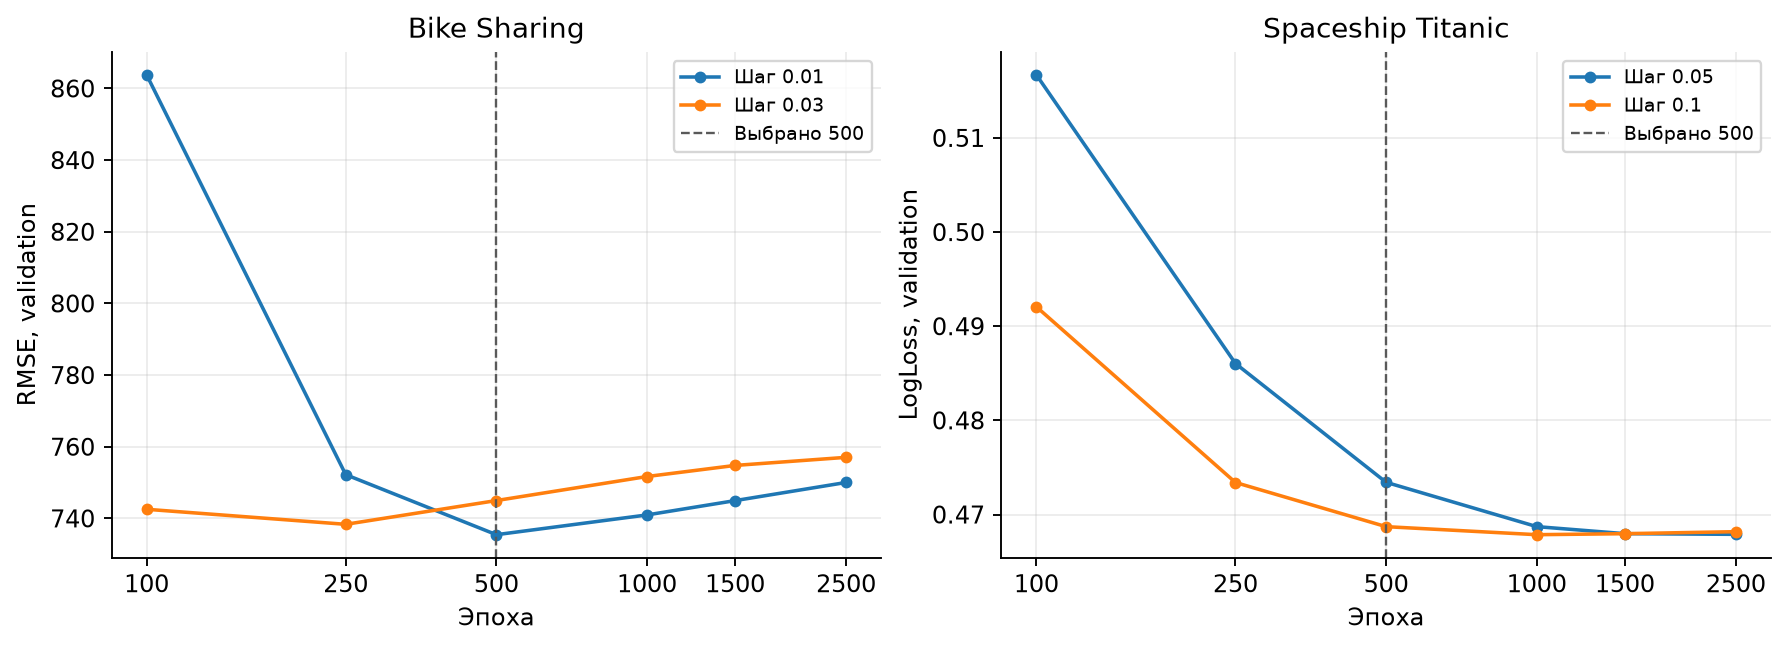
\includegraphics[width=\linewidth]{epoch_budget.png}
\caption{Validation RMSE и LogLoss для пробных шагов обучения}
\label{fig:epochs}
\end{figure}

Для Bike Sharing шаг 0,01 и 500 эпох дали RMSE 735,46. При том же шаге к 2500-й эпохе RMSE вырос до 750,04. Для Spaceship Titanic выбраны шаг 0,1 и 500 эпох: LogLoss 0,468712 находится в пределах допуска к минимуму 0,467859 на 1000-й эпохе. В последующих запусках четыре режима используют те же шаг и число эпох, нулевые начальные веса и одинаковые train и validation.

В Bike Sharing для $\lambda_1$ перебраны $0{,}25$, $1$, $4$, $16$, $64$, $256$, для $\lambda_2$ — $10^{-4}$, $10^{-3}$, $10^{-2}$, $0{,}1$, $0{,}5$. В Spaceship Titanic обе сетки состоят из степеней десяти от $10^{-5}$ до $10^{-1}$. Разные диапазоны учитывают масштаб MSE в квадрате единиц цели и безразмерный BCE. В ElasticNet проверяются все пары сеток. Лучший кандидат каждой семьи выбран по validation.

\subsection{Качество и величины весов}

На рис.~\ref{fig:reg-bike} и~\ref{fig:reg-ship} сопоставлены кривые четырёх режимов. Показана ошибка на данных без штрафа начиная со 125-й эпохи. Для Bike Sharing используется RMSE в арендах за день, для Spaceship Titanic — BCE. Кривые Spaceship Titanic почти совпадают из-за малых выбранных коэффициентов штрафа.

\begin{figure}[H]
\centering
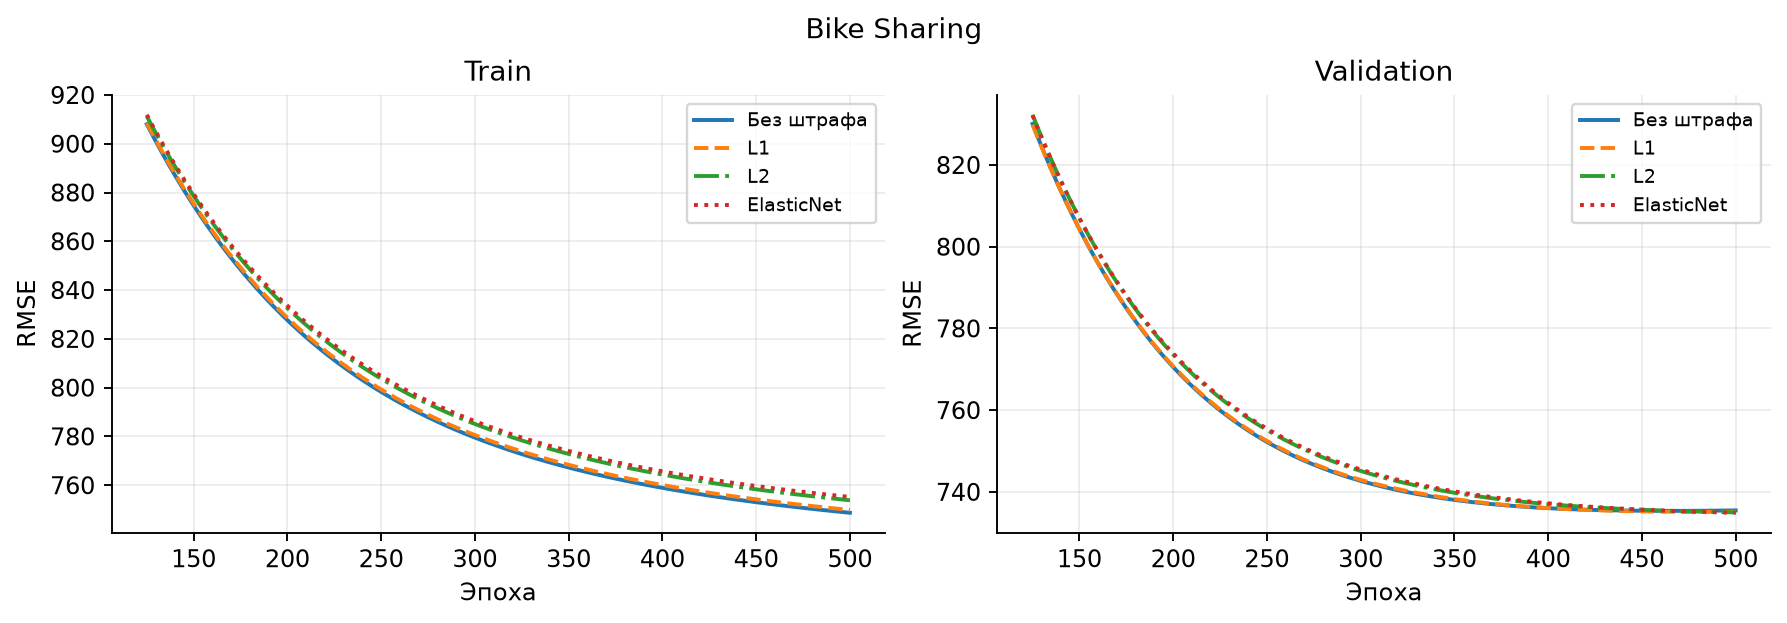
\includegraphics[width=\linewidth]{regularization_bike.png}
\caption{Bike Sharing. Ошибка на train и validation для четырёх режимов}
\label{fig:reg-bike}
\end{figure}

\begin{figure}[H]
\centering
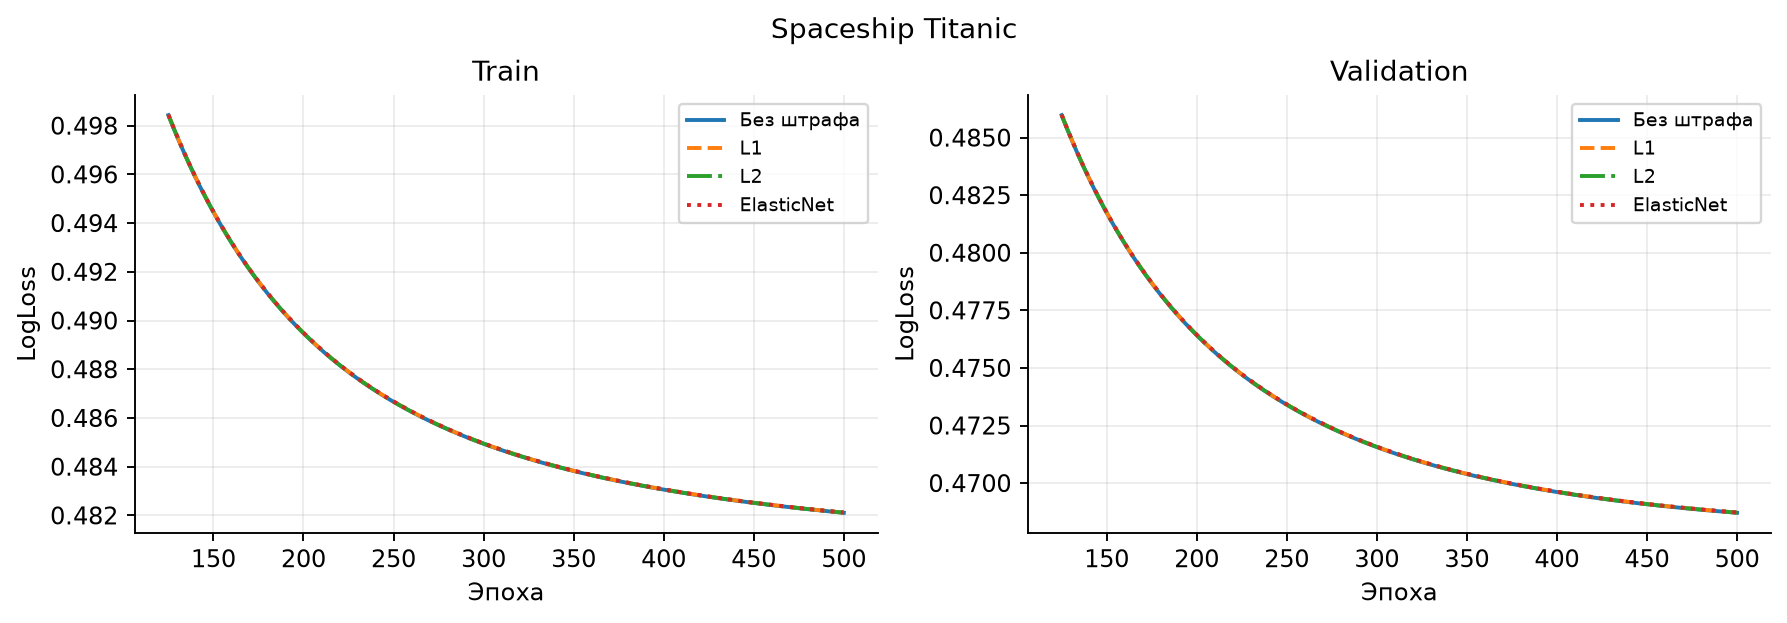
\includegraphics[width=\linewidth]{regularization_spaceship.png}
\caption{Spaceship Titanic. Ошибка на train и validation для четырёх режимов}
\label{fig:reg-ship}
\end{figure}

\begin{table}[H]
\centering
\caption{Коэффициенты и качество линейной регрессии}
\label{tab:bike}
\small
\begin{tabular}{lrrrrrr}
\toprule
Режим & $\lambda_1$ & $\lambda_2$ & RMSE val. & MAE test & RMSE test & $R^2$ test \\
\midrule
Без штрафа & 0 & 0 & 735,46 & 672,98 & 907,67 & 0,8117 \\
L1 & 4 & 0 & 735,13 & 675,40 & 910,72 & 0,8105 \\
L2 & 0 & 0,01 & 734,98 & 677,19 & 910,77 & 0,8105 \\
ElasticNet & 4 & 0,01 & 734,89 & 679,87 & 913,94 & 0,8091 \\
\bottomrule
\end{tabular}
\end{table}

\begin{table}[H]
\centering
\caption{Коэффициенты и качество логистической регрессии}
\label{tab:ship}
\small
\setlength{\tabcolsep}{4pt}
\begin{tabular}{lrrrrrrrr}
\toprule
Режим & $\lambda_1$ & $\lambda_2$ & LogLoss val. & Accuracy & Precision & Recall & F1 & LogLoss test \\
\midrule
Без штрафа & 0 & 0 & 0,468712 & 0,7729 & 0,7675 & 0,7877 & 0,7775 & 0,480348 \\
L1 & $10^{-5}$ & 0 & 0,468719 & 0,7729 & 0,7675 & 0,7877 & 0,7775 & 0,480354 \\
L2 & 0 & $10^{-5}$ & 0,468717 & 0,7729 & 0,7675 & 0,7877 & 0,7775 & 0,480352 \\
ElasticNet & $10^{-5}$ & $10^{-5}$ & 0,468725 & 0,7729 & 0,7675 & 0,7877 & 0,7775 & 0,480359 \\
\bottomrule
\end{tabular}
\par\smallskip Метрики по классу 1 рассчитаны на test при пороге вероятности 0,5.
\end{table}

Для Bike Sharing ElasticNet уменьшил validation RMSE на 0,57 аренды, однако test RMSE вырос на 6,26 (таблица~\ref{tab:bike}). В Spaceship Titanic лучший validation LogLoss у модели без штрафа. Положительные коэффициенты на нижней границе сетки дали близкие значения LogLoss и одинаковые пороговые метрики (таблица~\ref{tab:ship}). Большой штраф ухудшал приближение: L2 с $\lambda_2=0{,}5$ дал validation RMSE 1043,47 для Bike Sharing, а с $\lambda_2=0{,}1$ — validation LogLoss 0,535196 для Spaceship Titanic.

\begin{table}[H]
\centering
\caption{Величины 33 весов для каждой модели}
\label{tab:weights}
\small
\begin{tabular}{llrrrr}
\toprule
Данные & Режим & $\lVert w\rVert_1$ & $\lVert w\rVert_2$ & $\max_j|w_j|$ & Почти нулевых \\
\midrule
Bike Sharing & Без штрафа & 11\,689,28 & 3010,57 & 1972,19 & 0 \\
& L1 & 11\,378,82 & 2985,57 & 1971,87 & 1 \\
& L2 & 11\,347,23 & 2922,57 & 1924,22 & 0 \\
& ElasticNet & 11\,048,24 & 2898,34 & 1923,70 & 1 \\
\addlinespace
Spaceship Titanic & Без штрафа & 7,2550 & 1,7957 & 0,6955 & 5 \\
& L1 & 7,2471 & 1,7950 & 0,6953 & 6 \\
& L2 & 7,2526 & 1,7952 & 0,6953 & 5 \\
& ElasticNet & 7,2448 & 1,7945 & 0,6952 & 6 \\
\bottomrule
\end{tabular}
\end{table}

Порог почти нулевого веса равен 5 для Bike Sharing и 0,01 для Spaceship Titanic. Он относится к изменению ответа или логита при сдвиге преобразованного признака на единицу. В таблице~\ref{tab:weights} L1 и ElasticNet увеличили число малых весов на единицу в каждой модели. У L2 обе нормы уменьшились, число малых весов сохранилось. Фиксированный шаг субградиентного спуска допускает колебания малых весов около нуля.

\section{Метод ближайших соседей}

При обучении KNN сохраняет $X_{\text{train}}$ и $y_{\text{train}}$. Для запроса $x$ расстояние до объекта $u$ рассчитывается по одной из формул
\begin{equation}
d_{\mathrm{E}}(x,u)=\sqrt{\sum_{j=1}^{d}(x_j-u_j)^2},
\qquad
d_{\mathrm{M}}(x,u)=\sum_{j=1}^{d}|x_j-u_j|.
\label{eq:dist}
\end{equation}
Объекты сортируются по расстоянию. Для равных расстояний сохраняется порядок train. В классификации выбирается класс с наибольшим числом голосов среди $k$ соседей, при равном числе голосов — первый по алфавиту. В регрессии ответ равен среднему $y$ выбранных соседей. Расстояния рассчитываются тензорными операциями по~\eqref{eq:dist} блоками запросов.

Сравниваются $k\in\{1,3,5,9,15,25,41,65\}$ для каждого из двух расстояний с исходным масштабом и со стандартизацией. Один упорядоченный список длины 65 позволяет оценить каждое меньшее $k$ по его префиксу. При стандартизации числовой признак преобразуется как $(x_j-\mu_j)/\sigma_j$, где среднее и стандартное отклонение вычисляются на train. Для постоянного признака используется делитель 1, one-hot столбцы сохраняют масштаб 0/1.

\clearpage
\section{KNN-классификация Dry Bean}

В наборе~\cite{beans} 13\,611 измерений, 16 числовых признаков и семь сортов. После удаления 68 точных повторов осталось 13\,543 объекта. Выбор по Macro F1 даёт каждому сорту одинаковый вклад. По матрице ошибок $C$ с истинными классами по строкам для класса $c$ считаем $TP_c=C_{cc}$, $FN_c=\sum_j C_{cj}-TP_c$ и $FP_c=\sum_i C_{ic}-TP_c$. Затем
\[
\operatorname{Accuracy}=\frac{\sum_c C_{cc}}{\sum_{i,j}C_{ij}},\qquad
\operatorname{Macro\,F1}=\frac{1}{7}\sum_{c=1}^{7}\frac{2TP_c}{2TP_c+FP_c+FN_c}.
\]
При нулевом знаменателе вклад класса принимается равным нулю.

\begin{figure}[H]
\centering
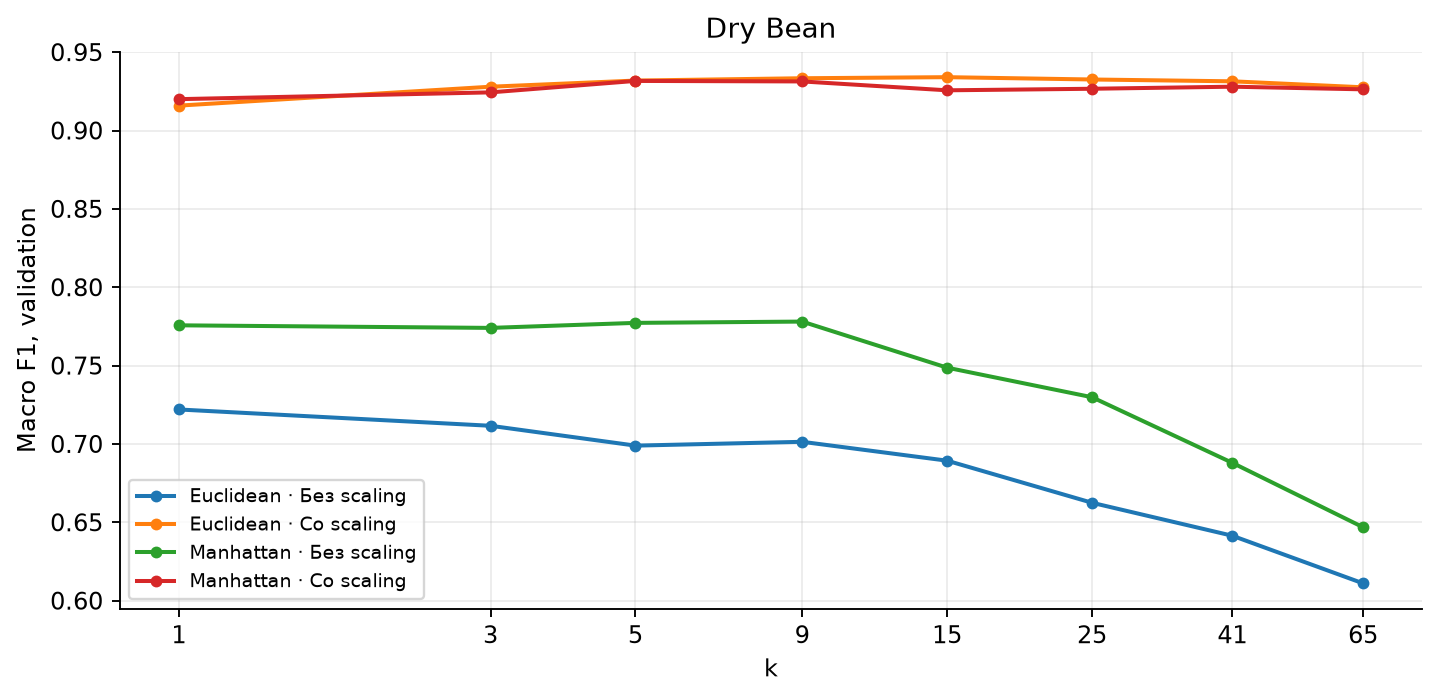
\includegraphics[width=.73\linewidth]{knn_dry_bean.png}
\caption{Dry Bean. Macro F1 по validation}
\label{fig:beans}
\end{figure}

\begin{table}[H]
\centering
\caption{Лучший $k$ в каждой комбинации на validation Dry Bean}
\label{tab:beans}
\small
\begin{tabular}{llrrr}
\toprule
Расстояние & Масштаб & $k$ & Accuracy & Macro F1 \\
\midrule
Euclidean & Исходный & 1 & 0,7218 & 0,7220 \\
Manhattan & Исходный & 9 & 0,7768 & 0,7781 \\
Euclidean & Стандартизированный & 15 & 0,9214 & 0,9340 \\
Manhattan & Стандартизированный & 5 & 0,9207 & 0,9317 \\
\bottomrule
\end{tabular}
\end{table}

При фиксированных Euclidean и $k=15$ scaling повысил validation Macro F1 с 0,6893 до 0,9340 (рис.~\ref{fig:beans}). Крупный численный масштаб площади и периметра доминировал над безразмерными признаками в исходном расстоянии. По таблице~\ref{tab:beans} для test выбран Euclidean со scaling и $k=15$. На 2712 объектах получены Accuracy 0,9229 и Macro F1 0,9353.

\begin{table}[H]
\centering
\caption{Матрица ошибок выбранного KNN на test Dry Bean}
\label{tab:confusion}
\small
\setlength{\tabcolsep}{3.5pt}
\begin{tabular}{lrrrrrrr}
\toprule
Истинный сорт & BARBUNYA & BOMBAY & CALI & DERMASON & HOROZ & SEKER & SIRA \\
\midrule
BARBUNYA & \textbf{237} & 0 & 16 & 0 & 3 & 2 & 7 \\
BOMBAY & 0 & \textbf{105} & 0 & 0 & 0 & 0 & 0 \\
CALI & 6 & 0 & \textbf{310} & 0 & 6 & 0 & 4 \\
DERMASON & 0 & 0 & 0 & \textbf{652} & 1 & 13 & 44 \\
HOROZ & 0 & 0 & 10 & 1 & \textbf{351} & 0 & 10 \\
SEKER & 0 & 0 & 0 & 11 & 0 & \textbf{383} & 12 \\
SIRA & 2 & 0 & 0 & 49 & 7 & 5 & \textbf{465} \\
\bottomrule
\end{tabular}
\par\smallskip В столбцах указаны предсказанные сорта.
\end{table}

В таблице~\ref{tab:confusion} основные ошибки приходятся на пару SIRA и DERMASON. Из 528 объектов SIRA 49 отнесены к DERMASON. В обратном направлении допущены 44 ошибки. Все 105 зёрен BOMBAY распознаны верно.

\section{KNN-регрессия Seoul Bike}

Набор~\cite{seoul} содержит 8760 часовых измерений за 365 дней, включая 295 часов закрытия проката. Признаки включают час, погоду, сезон, праздник и режим работы проката. Используются исторические значения погоды и предполагается известный режим работы. Дата служит для упорядочения и разбиения (таблица~\ref{tab:dates}).

\begin{table}[H]
\centering
\caption{Хронологические выборки Seoul Bike}
\label{tab:dates}
\small
\begin{tabular}{lccrr}
\toprule
Выборка & Начало & Конец & Дней & Часов \\
\midrule
Train & 01.12.2017 & 07.07.2018 & 219 & 5256 \\
Validation & 08.07.2018 & 18.09.2018 & 73 & 1752 \\
Test & 19.09.2018 & 30.11.2018 & 73 & 1752 \\
\bottomrule
\end{tabular}
\end{table}

\begin{figure}[H]
\centering
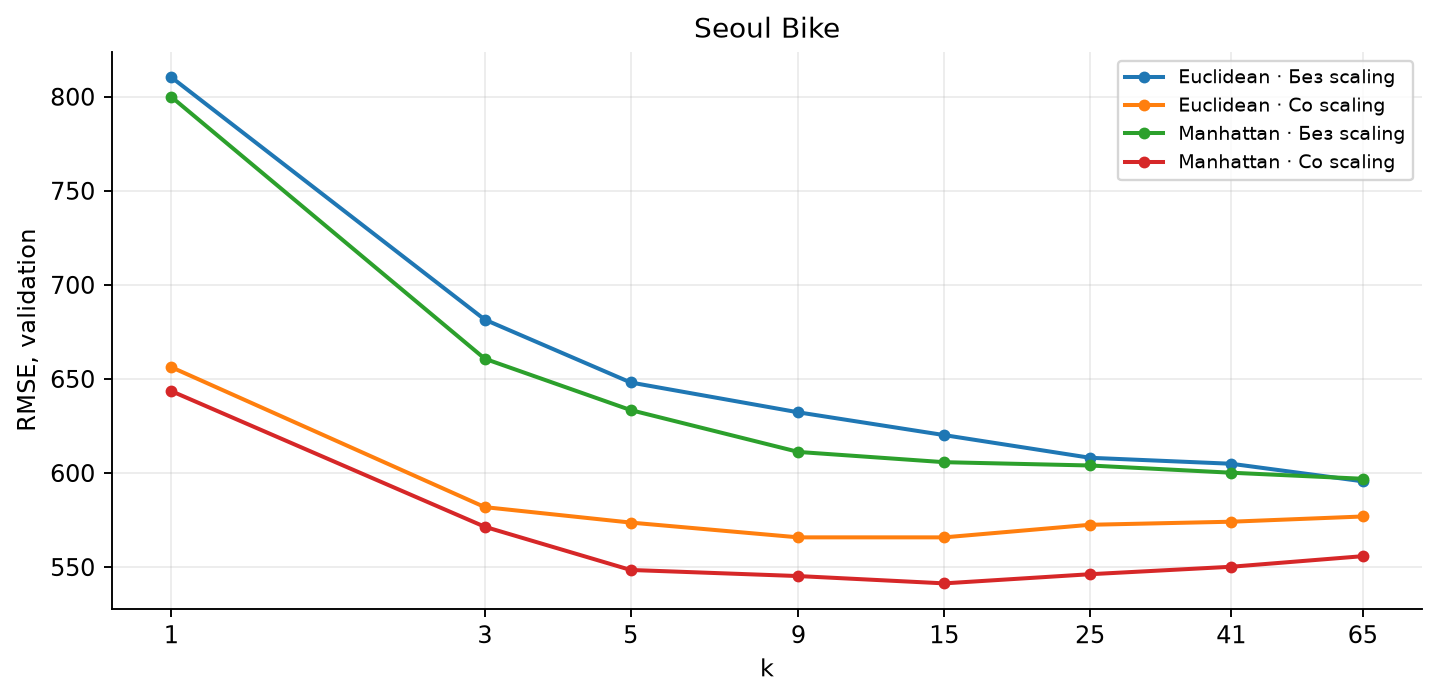
\includegraphics[width=.79\linewidth]{knn_seoul.png}
\caption{Seoul Bike. RMSE по validation}
\label{fig:seoul}
\end{figure}

\begin{table}[H]
\centering
\caption{Лучший $k$ в каждой комбинации на validation Seoul Bike}
\label{tab:seoul-val}
\small
\begin{tabular}{llrrrr}
\toprule
Расстояние & Масштаб & $k$ & MAE & RMSE & $R^2$ \\
\midrule
Euclidean & Исходный & 65 & 487,19 & 595,61 & 0,1234 \\
Manhattan & Исходный & 65 & 495,58 & 596,96 & 0,1194 \\
Euclidean & Стандартизированный & 15 & 443,06 & 565,82 & 0,2089 \\
Manhattan & Стандартизированный & 15 & 421,76 & 541,37 & 0,2758 \\
\bottomrule
\end{tabular}
\end{table}

При $k=15$ scaling уменьшил validation RMSE Manhattan с 605,78 до 541,37. На стандартизированных признаках Manhattan выиграл у Euclidean 24,45 аренды в RMSE при том же $k$ (рис.~\ref{fig:seoul}, таблица~\ref{tab:seoul-val}). Для test выбраны Manhattan, scaling и $k=15$. Базовый прогноз для каждого часа равен среднему по train: 600,92 аренды.

\begin{table}[H]
\centering
\caption{Метрики на test Seoul Bike}
\label{tab:seoul}
\small
\begin{tabular}{lrrr}
\toprule
Модель & MAE, аренды & RMSE, аренды & $R^2$ \\
\midrule
Среднее train & 507,69 & 632,88 & $-0{,}0648$ \\
KNN & 342,47 & 510,08 & 0,3084 \\
\bottomrule
\end{tabular}
\end{table}

KNN снизил test RMSE на 19,4\% относительно baseline (таблица~\ref{tab:seoul}). У baseline $R^2<0$: среднее train отличается от среднего на test, около 757 аренд. В test 223 часа закрытия проката, в validation — 24. Осенний сезон отсутствует в train, поэтому его one-hot блок на test состоит из нулей. Результат описывает прогноз при переходе к конкретному более позднему периоду.

\begin{samepage}
\section{Выводы}

Штрафы уменьшили нормы весов обеих регрессий. При выбранных коэффициентах L1 и ElasticNet дали больше почти нулевых весов. Выигрыш ElasticNet на validation Bike Sharing был мал и не повторился на test. В логистической регрессии минимальный LogLoss получен без штрафа. Для KNN стандартизация улучшила качество на обоих наборах, а выбранное расстояние зависело от задачи. На Dry Bean получен Macro F1 0,9353, на Seoul Bike KNN снизил MAE и RMSE и повысил $R^2$ относительно постоянного прогноза.

\end{samepage}
\begin{thebibliography}{4}\raggedright
\bibitem{bike} Bike Sharing Dataset. \href{https://www.kaggle.com/datasets/marklvl/bike-sharing-dataset}{Kaggle}.
\bibitem{ship} Spaceship Titanic. \href{https://www.kaggle.com/competitions/spaceship-titanic/data}{Kaggle}.
\bibitem{beans} Koklu M., Özkan I. A. Dry Bean Dataset. UCI Machine Learning Repository. \href{https://doi.org/10.24432/C50S4B}{DOI 10.24432/C50S4B}.
\bibitem{seoul} Seoul Bike Sharing Demand. UCI Machine Learning Repository. \href{https://doi.org/10.24432/C5F62R}{DOI 10.24432/C5F62R}.
\end{thebibliography}

\end{document}
